\documentclass{article}
\usepackage[utf8]{inputenc}  % Para caracteres acentuados
\usepackage{booktabs}        % Para \toprule, \midrule, \bottomrule
\usepackage{graphicx}        % Para inserir figuras
\usepackage{float}           % Para usar [H] e fixar posição da figura
\usepackage{lipsum}          % Para texto de exemplo (opcional)

\begin{document}
	
	% --- Espaço para texto introdutório ---
	
	
	% --- Tabela de Frequências discretas template---
	\section*{Tabela de Frequências}
	
	
	% --- Tabela de Frequências contínua template---
	\begin{table}[H]
\centering
\caption{Distribuição de frequências referentes ao tempo de convergência (em segundos) do modelo de Machine Learning para classificação de Raio-X}
\begin{tabular}{cccccc}
\toprule
Intervalo (LI $\vdash$ LS) & Xi & Fi & Fr & Fp (\%) \\
\midrule
1.7 $\vdash$ 4.1   & 2.9  & 5  & 0.1389 & 13.89 \\
4.1 $\vdash$ 6.5   & 5.3  & 13 & 0.3611 & 36.11 \\
6.5 $\vdash$ 8.9   & 7.7  & 7  & 0.1944 & 19.44 \\
8.9 $\vdash$ 11.3  & 10.1 & 5  & 0.1389 & 13.89 \\
11.3 $\vdash$ 13.7 & 12.5 & 4  & 0.1111 & 11.11 \\
13.7 $\vdash$ 16.1 & 14.9 & 2  & 0.0556 & 5.56 \\
\midrule
TOTAL & - & 36 & 1.00 & 100.00 \\
\bottomrule
\end{tabular}
\label{tab:freq_intervalos_total}
\end{table}


	% --- Espaço para análise ou comentários ---
\section*{Análise}
b) De acordo com a tabela 1, 6 simulações possuem tempo de convergência
de pelo menos 11,3 segundos.\newline\newline
c) De acordo com a tabela 1, 13,89 + 36,11 + 19,44 = 69,44\% das simulações apresentam tempo de convergência menores que 8,9 segundos. \newline\newline
d) De acordo com a tabela 1, 13,89 + 36,11 + 19,44/2 = 59,72\% 
das simulações apresentam tempo de convergência menores que 7,7 segundos.

	
	
	% --- Gráfico centralizado template---
	\section*{Gráfico}
	\begin{figure}[H]
		\centering
		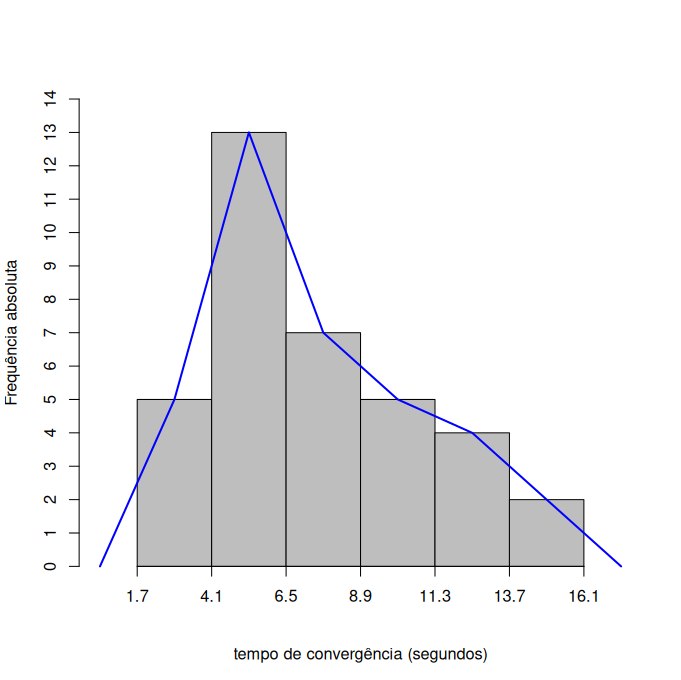
\includegraphics[width=0.7\textwidth]{/home/thallysson/Área de trabalho/Disciplinas/Estatistica/latex/graficos/grafico_atividade3_ex2.png} % substitua pelo arquivo do seu gráfico
		\caption{Histograma da distribuição de frequências referentes ao tempo de convergência (em segundos) do modelo de Machine Learning para classificação de Raio-X}
		\label{fig:grafico_filhos}
	\end{figure}
	
	\section*{Análise}
	e) O gráfico da figura 1 é assimétrico a esquerda
	

	
	
\end{document}

